%  Template for ICASSP-2021 paper; to be used with:
%          spconf.sty  - ICASSP/ICIP LaTeX style file, and
%          IEEEbib.bst - IEEE bibliography style file.
% --------------------------------------------------------------------------
\documentclass{article}
\usepackage{spconf,amsmath,graphicx,hyperref}

% Example definitions.
% --------------------
\def\x{{\mathbf x}}
\def\L{{\cal L}}

% Title.
% ------
\title{AIML 425 Assignemnt 4}
%
% Single address.
% ---------------
\name{Quan Zhao (Student ID: 300471028)}
%\name{Author(s) Name(s)\thanks{Thanks to XYZ agency for funding.}}
\address{Victoria University of Wellington}


\begin{document}
%\ninept
%
\maketitle
%
\section{Introduction}
\label{sec:intro}

An autoencoder is a type of artificial neural network primarily used for unsupervised learning tasks, such as data compression and noise reduction. Its architecture is tailored to learn efficient codings or representations of input data, often for dimensionality reduction or for learning generative models of data. In this report, I will elucidate my understanding of autoencoders by training one on 3D data uniformly distributed over the surface of a cube. Subsequently, I will introduce a method to control the distribution of the latent (bottleneck) variable and incorporate iid Gaussian noise to this latent variable with an adjustable, non-learned SNR. We will then discuss the characteristics of the reconstructions obtained at various SNRs and dimensionalities of the latent vector. Finally, we will choose a quality measure to quantify the generative performance of the autoencoder.

\section{THEORY}
\label{sec:theory}

\subsection{Variational autoencoder (VAE)}
\label{ssec:vae}

Variational Autoencoders (VAEs) \cite{kingma2013auto} are a type of generative model that builds upon traditional autoencoders by incorporating probabilistic layers and a distinct regularization term. While standard autoencoders learn deterministic encodings of the input data, VAEs are designed to learn probabilistic mappings. As a result, the latent space of a VAE is structured to follow a specific probability distribution, most commonly a Gaussian distribution.

\begin{equation}
  \text{ELBO}(\theta, \phi; x) = \text{E}_{q_\phi(z|x)}[\log p_\theta(x|z)] - \text{KL}(q_\phi(z|x) || p(z))
  \end{equation}
  

\subsection{Signal-to-Noise Ratio (SNR)}
\label{ssec:snr}

The Signal-to-Noise Ratio, commonly abbreviated as SNR, is a measure used to quantify the level of a desired signal relative to the level of background noise. 
In the context of digital signals and data processing, the SNR \cite{vincent2008extracting} provides insights into the clarity and quality of a signal amidst the presence of noise.

In autoencoders, the latent or bottleneck variable captures the compressed representation of the input data. By introducing noise, specifically iid (independent and identically distributed) Gaussian noise, to this latent space, one can simulate real-world scenarios where data might be corrupted or perturbed. This process can also act as a form of regularization, potentially improving the generalization capability of the autoencoder.

Why Gaussian Noise? 
Gaussian noise, characterized by its bell-shaped probability distribution, is a common choice due to its natural occurrence in many real-world scenarios. When noise is added to the latent space of an autoencoder, it's essential that this noise doesn't dominate the original signal. The SNR can help in quantifying the balance between the latent variable's information (signal) and the introduced noise.

\subsection{Earth Mover's Distance (EMD)}
\label{ssec:emd}

The Earth Mover's Distance, commonly referred to as EMD or Wasserstein distance\cite{tolstikhin2017wasserstein}, is a metric that quantifies the dissimilarity between two probability distributions over a given space. Originating from the fields of transportation and economics, EMD has found extensive applications in computer vision, machine learning, and image retrieval due to its sensitivity to the spatial distribution of data points.

Imagine two distinct piles of soil representing two distributions. The goal is to reshape one pile to match the other. EMD measures the least amount of "work" required to achieve this, where "work" is determined by the product of the soil amount and the distance it's moved.

For two distributions 
$P$ and 
$Q$, EMD is the minimal cumulative cost to transfer mass from points in 
$P$ to points in 
$Q$. This transformation can be represented as a linear programming problem, though faster algorithms and approximations have been developed for specific scenarios.


\section{RESULTS}
\label{sec:results}

\subsection{Data}
\label{ssec:data}

This work is based on the data which uniformly distributed over the surface of a cube. 
The data distribution is showing in Figure $\ref{fig:data}$.

\begin{figure}[htb]
  \begin{minipage}[b]{1.0\linewidth}
    \centering
    \centerline{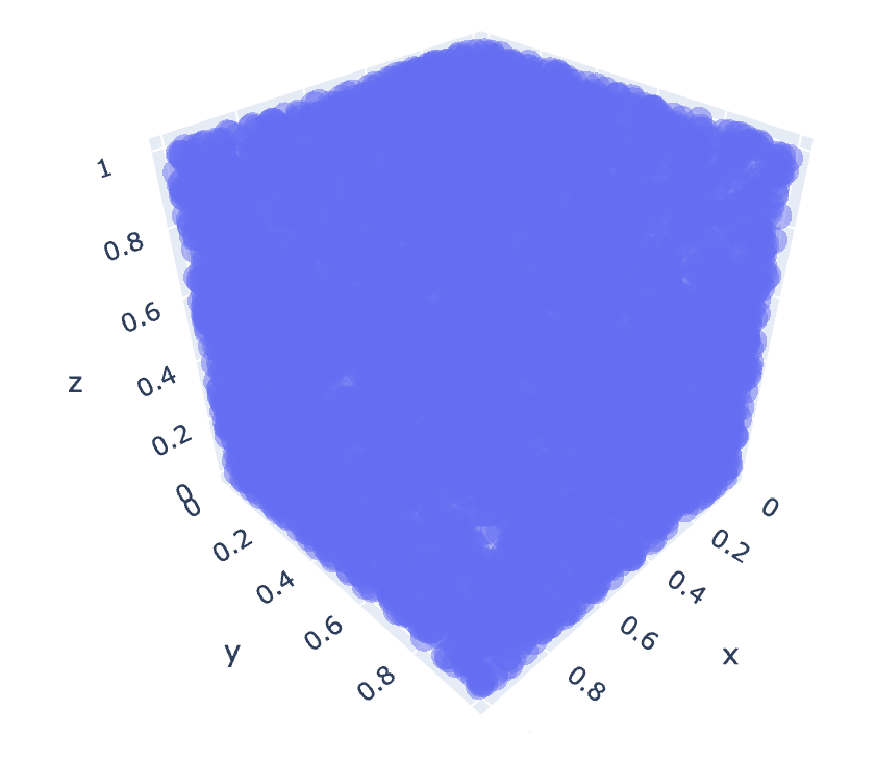
\includegraphics[width=7.0cm]{images/data}}
  \end{minipage}
  \caption{3D data that are uniformly distributed over the surface of a cube}
  \label{fig:data}
  %
  \end{figure}

\subsection{Basic autoencoder}
\label{ssec:basicautoencoder}

We began by training the autoencoder using a basic approach, incorporating both an encoder and a decoder with the Mean Squared Error (MSE) as the objective function. After adjusting the dimension of the latent variables and visualizing the decoder output, we found that the model performed optimally with 7 latent variables. However, we also observed that the distribution of each latent variable was unstable, as shown in Figure $\ref{fig:basic}$.

\subsubsection{Interpretation of the MSE objective function which used in autoencoder}
\label{sssec:mse}
The MSE objective function in an autoencoder can be seen as a maximum likelihood estimator under the assumption that the reconstruction error is Gaussian noise with a fixed variance. This probabilistic interpretation provides a deeper understanding of why MSE is a natural choice for many regression and reconstruction tasks: it corresponds to the assumption of Gaussian noise, which is a common and often reasonable assumption about the nature of errors in many real-world scenarios.

\begin{figure}[htb]
  \begin{minipage}[b]{1.0\linewidth}
    \centering
    \centerline{\includegraphics[width=7.0cm]{images/basic_r1}}
  %  \vspace{1.5cm}
    \centerline{(a) round 1}\medskip
  \end{minipage}
  \hfill
  \begin{minipage}[b]{1.0\linewidth}
    \centering
    \centerline{\includegraphics[width=7.0cm]{images/basic_r2}}
  %  \vspace{1.5cm}
    \centerline{(b) round 2 }\medskip
  \end{minipage}
  %
  \caption{distribution of latent variables}
  \label{fig:basic}
  %
  \end{figure}

\subsection{Control the distribution of latent variable}
\label{ssec:VAE}

To address the instability in the latent variable distribution observed in the basic autoencoder, we opted for the Variational Autoencoder (VAE). This allowed us to better control the distribution of the latent (bottleneck) variables. Subsequently, we introduced iid Gaussian noise to the latent (bottleneck) variable, using an adjustable (non-learned) SNR.
\subsection{attributes of the reconstruction that you obtain at various SNRs and dimensionalities of the latent vector (select a range of interesting settings)}
\label{ssec:discuss}

We experimented with various parameter values:

SNR values of 5, 10, 20, 50, and 100.
Latent dimensionalities of 2, 3, 5, 7, and 10.
Figure $\ref{fig:discuss}$ illustrates that when the latent dimension is low, the latent space cannot capture all the information from the input, resulting in a reconstructed output that appears banded. Conversely, with a higher latent dimension, more information is represented.

Regarding SNR, a lower value results in a more compact representation, whereas a higher value leads to a more scattered distribution.
\begin{figure}[htb]
  \centering
  % First row
  \begin{minipage}[b]{0.3\linewidth}
    \centering
    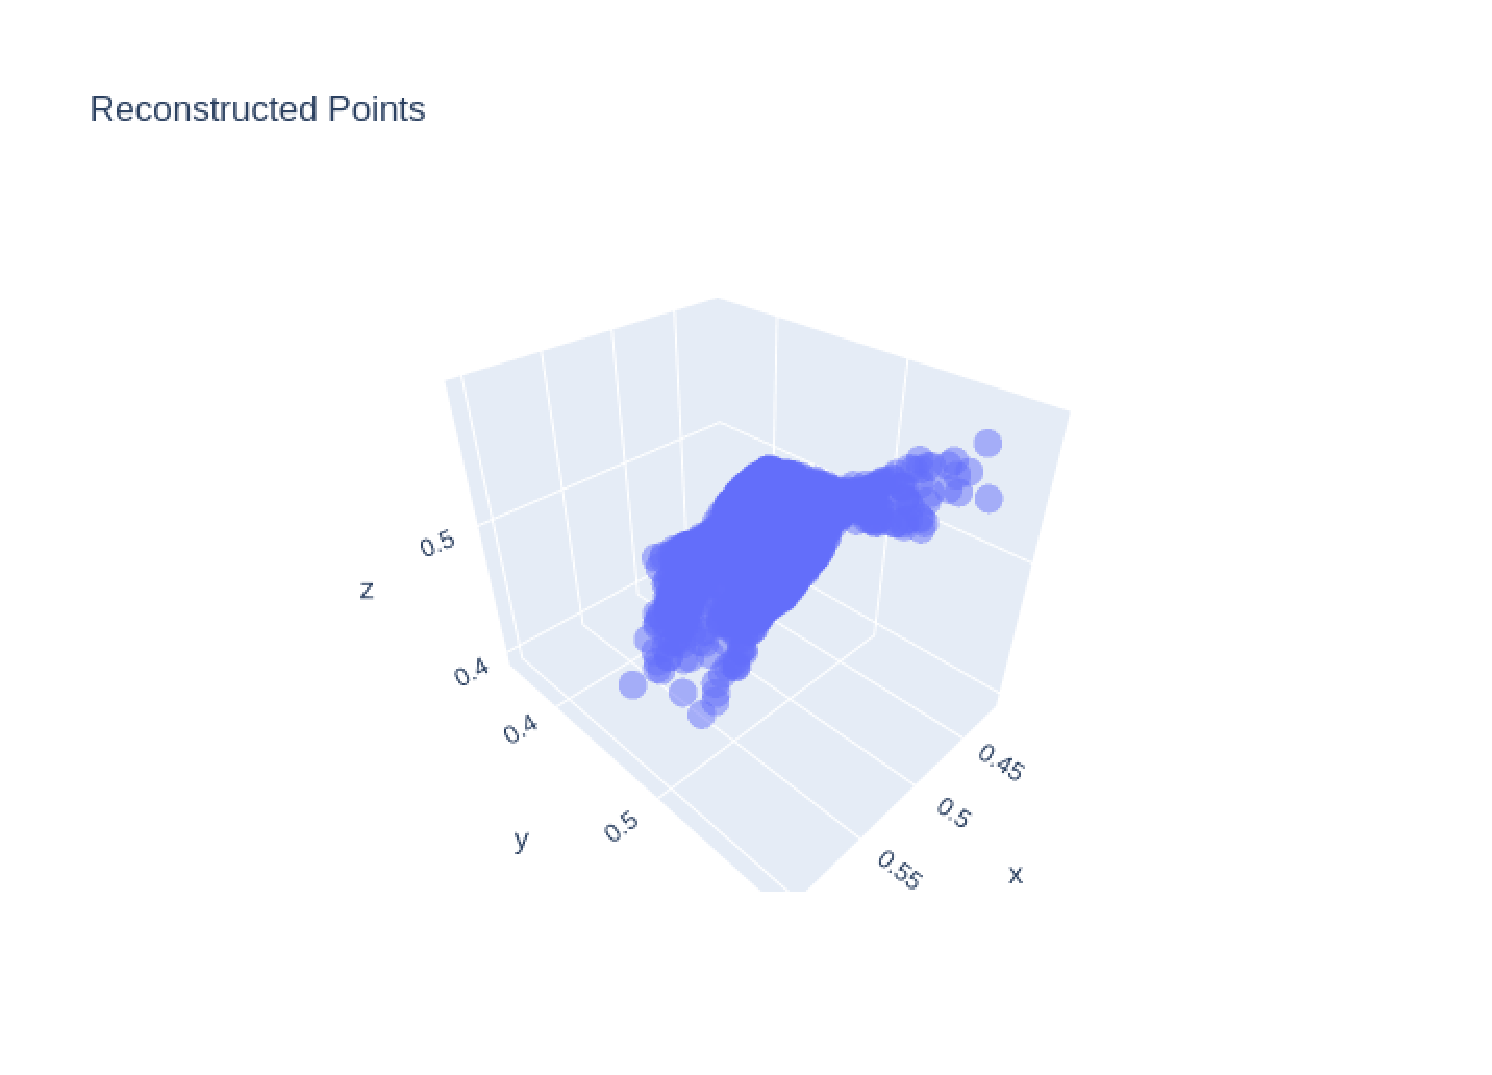
\includegraphics[width=3.0cm]{images/reconstructed_2_5}
    \centerline{(a) dim 2, snr 5}\medskip
  \end{minipage}
  \hfill
  \begin{minipage}[b]{0.3\linewidth}
    \centering
    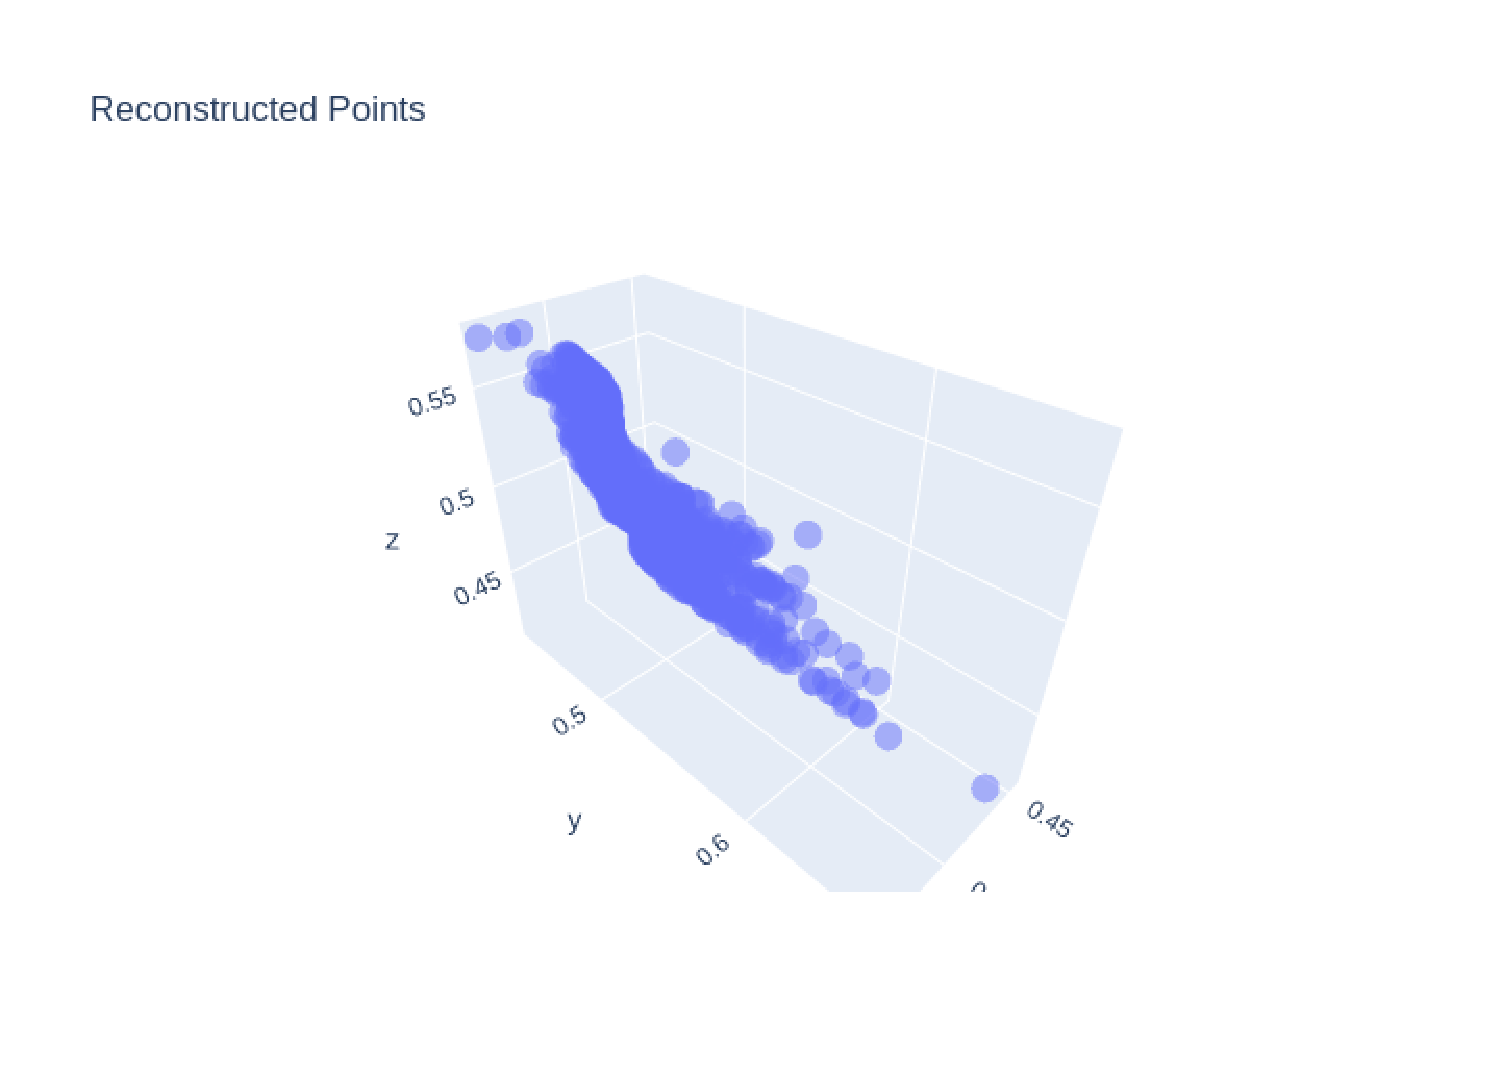
\includegraphics[width=3.0cm]{images/reconstructed_2_50}
    \centerline{(a) dim 2, snr 50}\medskip
  \end{minipage}
  \hfill
  \begin{minipage}[b]{0.3\linewidth}
    \centering
    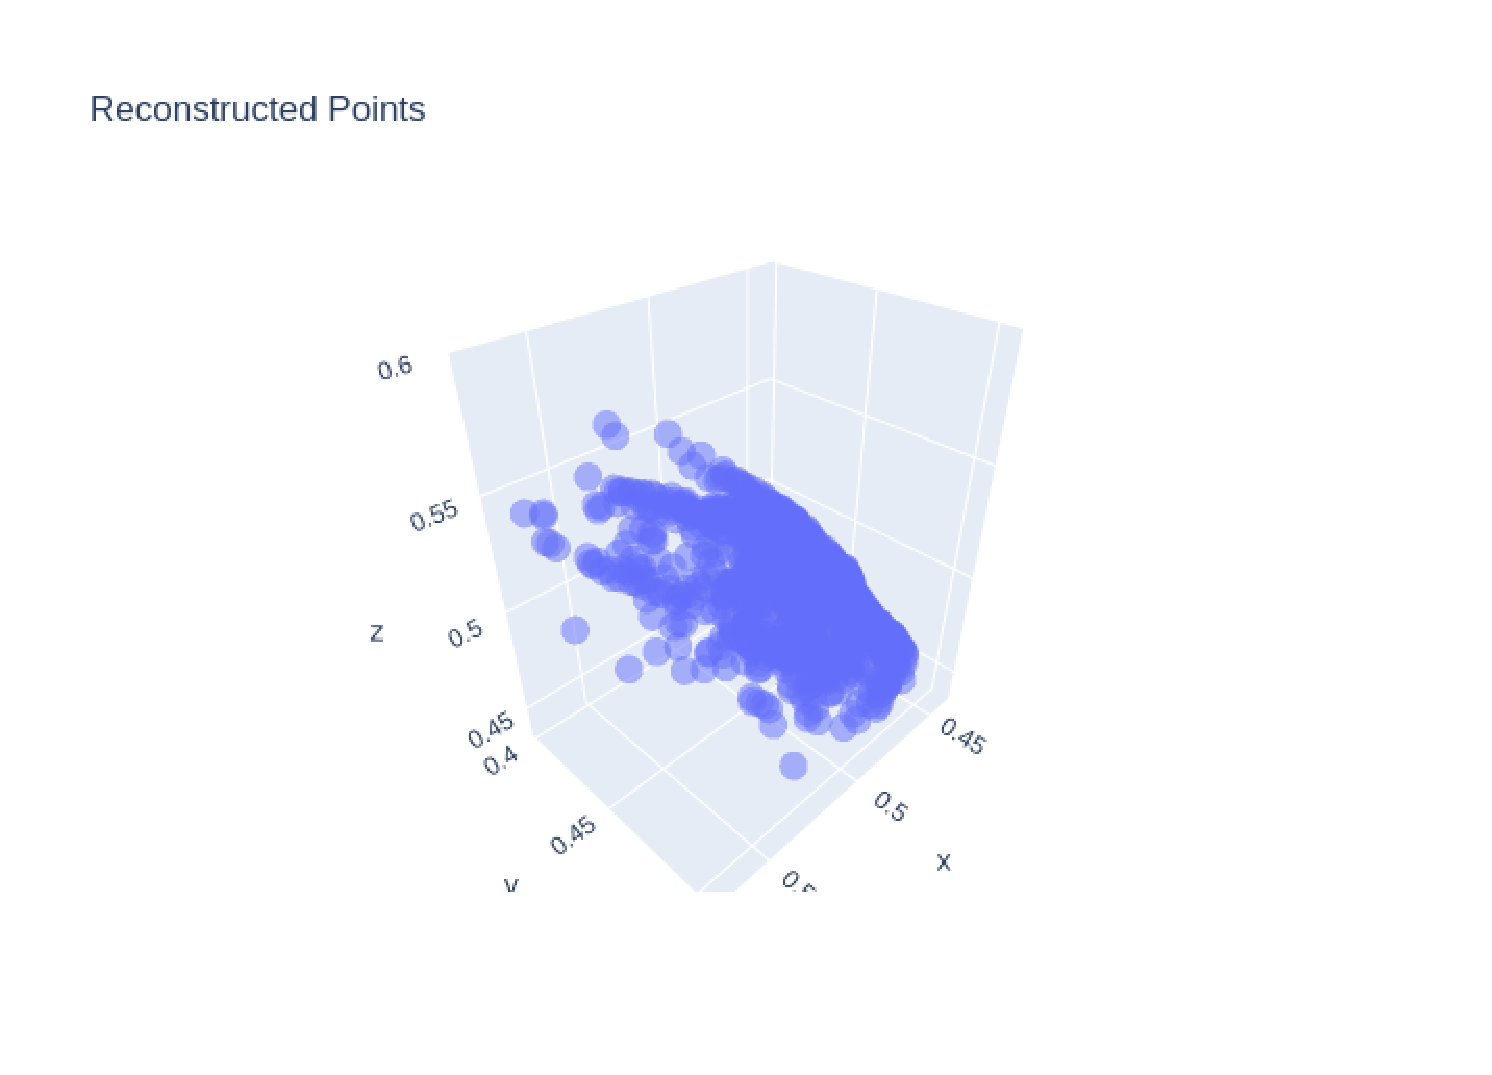
\includegraphics[width=3.0cm]{images/reconstructed_2_100}
    \centerline{(c) dim 2, snr 100}\medskip
  \end{minipage}
  
  % \vspace{1cm} % Add some vertical space between the rows
  
  % Second row
  \begin{minipage}[b]{0.3\linewidth}
    \centering
    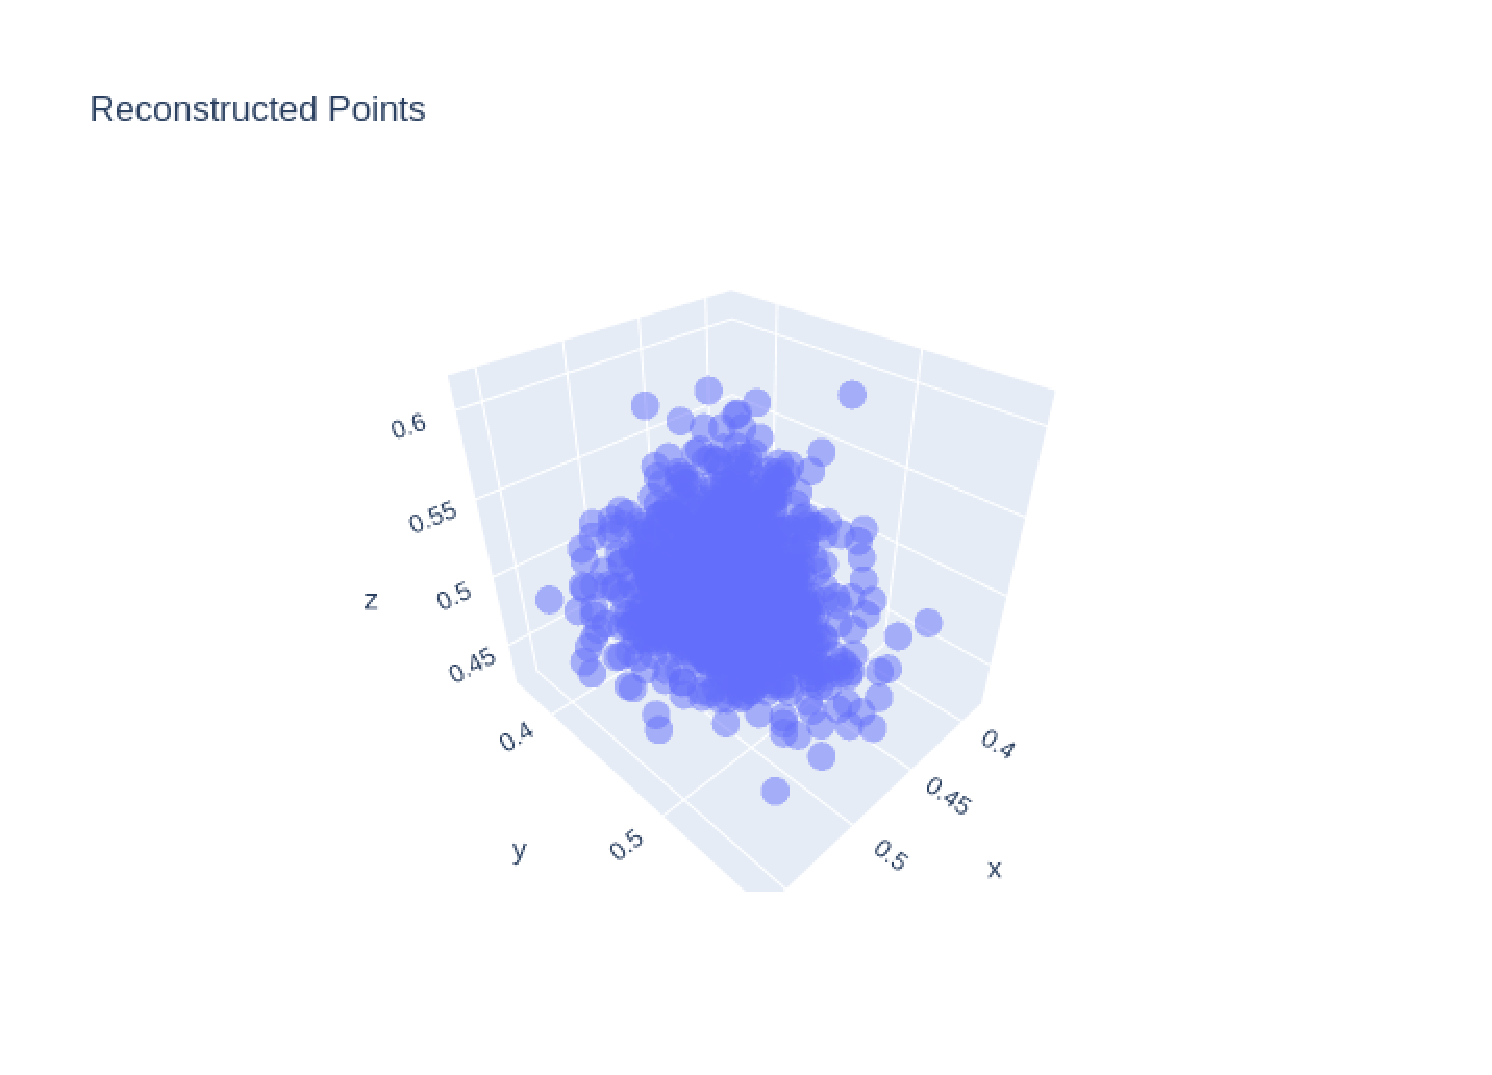
\includegraphics[width=3.0cm]{images/reconstructed_10_5}
    \centerline{(d) dim 10, snr 5}\medskip
  \end{minipage}
  \hfill
  \begin{minipage}[b]{0.3\linewidth}
    \centering
    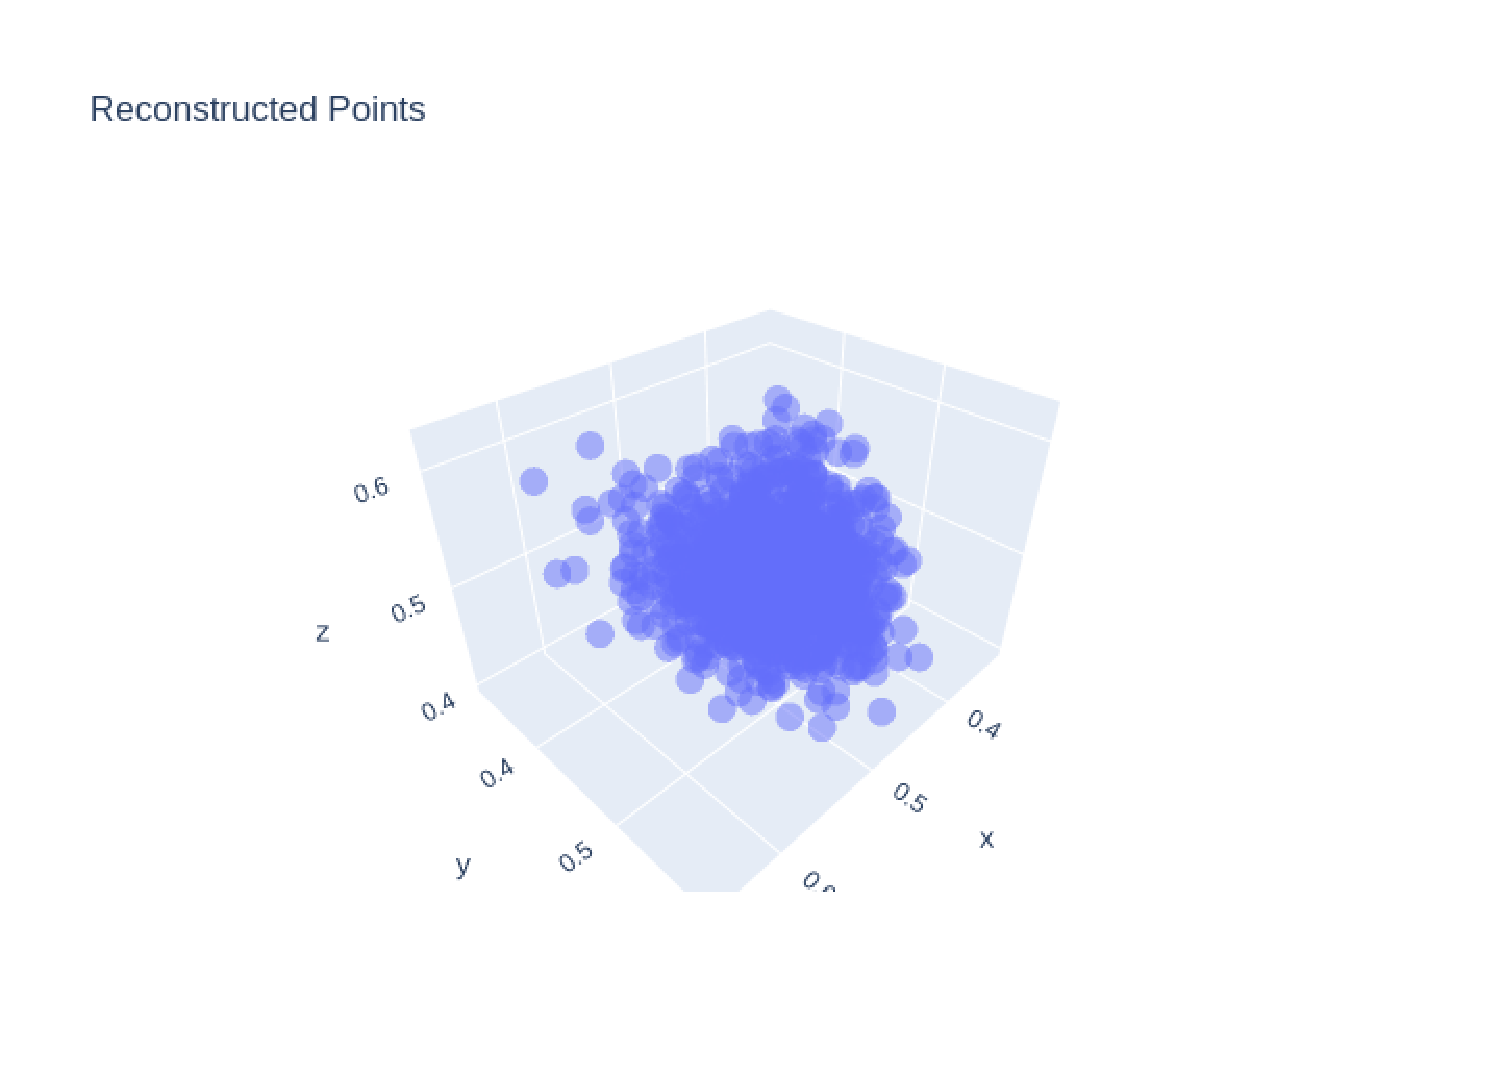
\includegraphics[width=3.0cm]{images/reconstructed_10_50}
    \centerline{(e) dim 10, snr 50}\medskip
  \end{minipage}
  \begin{minipage}[b]{0.3\linewidth}
    \centering
    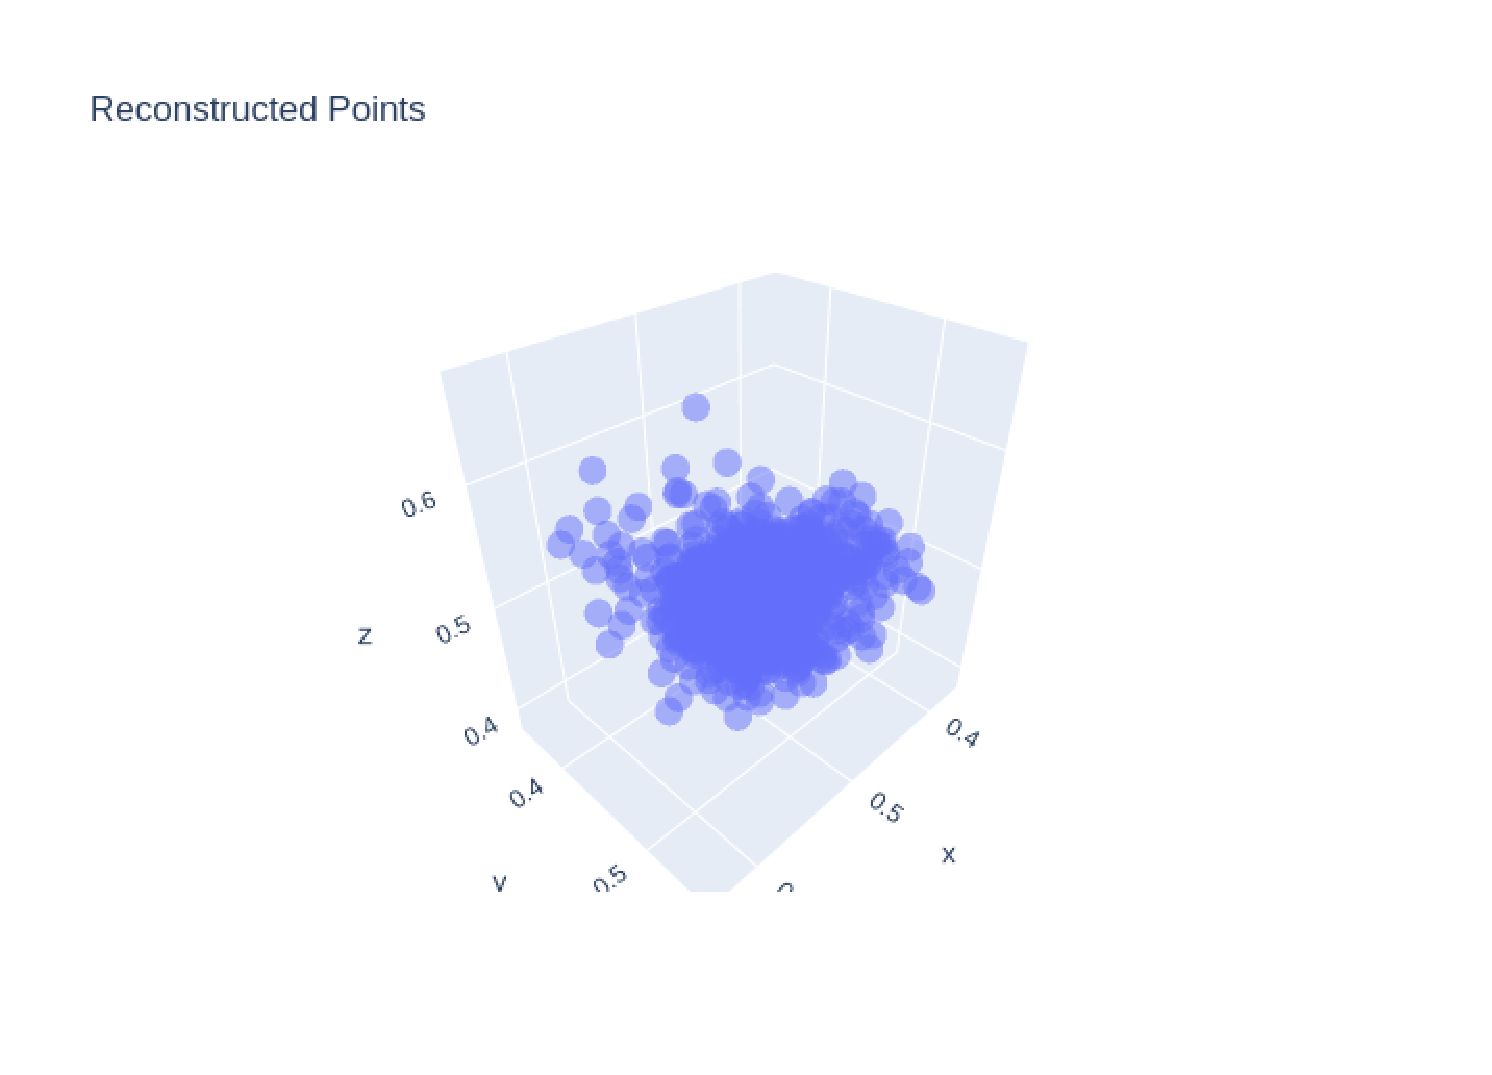
\includegraphics[width=3.0cm]{images/reconstructed_10_100}
    \centerline{(f) dim 10, snr 100}\medskip
  \end{minipage}
  
  \caption{reconstructed plot with different latent dimension and SNR}
  \label{fig:discuss}
\end{figure}

\subsection{quality measure and quantify performance }
\label{ssec:measure}

For 3D point clouds, such as the surface of a cube, metrics like the Chamfer distance or EMD are commonly employed. In this study, we chose the Earth Mover's Distance (EMD) to evaluate the model's performance.

Based on the EMD score, we selected a latent dimensionality of 10 and an SNR of 50 from the previously given range.
\section{CONCLUSION}
\label{sec:conclusion}

Autoencoders are popular in machine learning approaches. Their applications range from dimensionality reduction and data compression to anomaly detection. In this work, we trained a basic autoencoder and identified an instability in the latent distribution. To address this issue, we employed a Variational Autoencoder (VAE) and utilized SNR to smooth the latent space. Finally, we adopted the Earth Mover's Distance (EMD) as a metric to evaluate model performance and fine-tune the parameters.


\section{STATEMENT OF ALL TOOLS USED}
\label{sec:statementofalltoolsused}

In this work, we used Pytorch geometric package to generate data, create, train models. 
The Plotly package helped us visualize in 3D. 

Source codes are published in github: 
$\href{https://github.com/felixzhao/AIML425-ASSN-3/blob/main/AIML425_Assignment_3.ipynb}{URL}$
 (runable in google colab)



% To start a new column (but not a new page) and help balance the last-page
% column length use \vfill\pagebreak.
% -------------------------------------------------------------------------
%\vfill
%\pagebreak

\vfill\pagebreak

% References should be produced using the bibtex program from suitable
% BiBTeX files (here: strings, refs, manuals). The IEEEbib.bst bibliography
% style file from IEEE produces unsorted bibliography list.
% -------------------------------------------------------------------------
\bibliographystyle{IEEEbib}
\bibliography{strings,refs}

\end{document}
